\chapter{细胞周期与有丝分裂}\label{ch:g11:cell-cycle-mitosis}

取洋葱根尖压片，染色后观察：
在数以百计、\omterm{def:g10:cells-common-unit:organelle}{细胞核}呈圆形的静止\omterm{def:g10:cells-common-unit:cell}{细胞}中，少数
\omterm{def:g10:cells-common-unit:cell}{细胞}呈现另一番景象——深色的 X 形\omterm{def:g11:cell-cycle-mitosis:chromosome}{染色体}聚集在\omterm{def:g10:cells-common-unit:cell}{细胞}中央，或两组
\omterm{def:g11:cell-cycle-mitosis:chromosome}{染色体}被拉向两端，或两个小\omterm{def:g10:cells-common-unit:organelle}{细胞核}
之间正在形成\omterm{def:g10:cells-common-unit:organelle}{细胞壁}。你看到的是\omterm{def:g10:cells-common-unit:cell}{细胞}分裂
恰好停留在不同时刻的画面，它发生在每天生长一毫米的组织中。每一次分裂
都把两套完整、相同的\omterm{def:g11:cell-cycle-mitosis:chromosome}{染色体}分给两
个子\omterm{def:g10:cells-common-unit:cell}{细胞}。本章追踪一个\omterm{def:g10:cells-common-unit:cell}{细胞}走完一个完整周期，并
仔细观察\omterm{def:g11:cell-cycle-mitosis:chromosome}{染色体}被分配的那段时间。

\section{细胞周期}

\begin{definition}[细胞周期]\label{def:g11:cell-cycle-mitosis:cycle}
称\emph{细胞周期}\index{细胞周期}为\omterm{def:g10:cells-common-unit:cell}{细胞}从
由分裂产生之时起，到自身再分裂为两个\omterm{def:g10:cells-common-unit:cell}{细胞}为止的一系列事件。它
包括\emph{间期}，\omterm{def:g10:cells-common-unit:cell}{细胞}在此期间生长并
复制 \omterm{def:g10:universal-dna:information}{DNA}；另一阶段是\emph{M 期}，\omterm{def:g10:cells-common-unit:organelle}{细胞核}在其中
先分裂（\emph{有丝分裂}\index{有丝分裂}），随后\omterm{def:g10:cells-common-unit:cell}{细胞质}
分裂（\emph{胞质分裂}）。间期分为三个阶段：$\mathrm{G_1}$
（生长），S 期（\omterm{def:g10:universal-dna:information}{DNA} 复制，见\cref{ch:g11:dna-replication}）和
$\mathrm{G_2}$（分裂准备）。
\end{definition}

\begin{omfigure}
\begin{tikzpicture}[font=\small]
  % pie: G1 11h, S 8h, G2 4h, M 1h  (24h) -> angles: G1 165°, S 120°, G2 60°, M 15°
  \fill[omDef!30] (0,0) -- (90:2.2) arc (90:-75:2.2) -- cycle;
  \fill[omProp!35] (0,0) -- (-75:2.2) arc (-75:-195:2.2) -- cycle;
  \fill[omMeth!35] (0,0) -- (-195:2.2) arc (-195:-255:2.2) -- cycle;
  \fill[omThm!50] (0,0) -- (-255:2.2) arc (-255:-270:2.2) -- cycle;
  \draw[thick] (0,0) circle (2.2);
  \foreach \a in {90,-75,-195,-255} \draw[thick] (0,0) -- (\a:2.2);
  \node at (10:1.3) {$\mathrm{G_1}$};
  \node at (-135:1.3) {S};
  \node at (-225:1.35) {$\mathrm{G_2}$};
  \node[anchor=south east] at (-262:2.35) {M};
  \node[anchor=west, align=left] at (2.6,1.3) {$\mathrm{G_1}$：生长，约 \qty{11}{h}};
  \node[anchor=west, align=left] at (2.6,0.5) {S：DNA 复制，\qty{8}{h}};
  \node[anchor=west, align=left] at (2.6,-0.3) {$\mathrm{G_2}$：准备，\qty{4}{h}};
  \node[anchor=west, align=left] at (2.6,-1.1) {M：有丝分裂与胞质分裂，\qty{1}{h}};
  \draw[->, thick] (100:2.5) arc (100:130:2.5);
\end{tikzpicture}

{\small 典型分裂的人体\omterm{def:g10:cells-common-unit:cell}{细胞}的\omterm{def:g11:cell-cycle-mitosis:cycle}{细胞周期}约为 24
小时。间期（$\mathrm{G_1}$、S、$\mathrm{G_2}$）占其中 23 小时，
分裂本身占 1 小时。许多\omterm{def:g10:cells-common-unit:cell}{细胞}在
$\mathrm{G_1}$ 期后即退出周期，不再分裂。}
\end{omfigure}

\begin{proposition}[细胞周期中的 DNA]\label{prop:g11:cell-cycle-mitosis:dna}
设 $q$ 为\omterm{def:g10:cells-common-unit:cell}{细胞}刚分裂后\omterm{def:g10:cells-common-unit:organelle}{细胞核}中 \omterm{def:g10:universal-dna:information}{DNA} 的量。它
保持为 $q$ 直至 $\mathrm{G_1}$ 期结束，S 期中随\omterm{def:g11:cell-cycle-mitosis:chromosome}{染色体}复制逐渐升至 $2q$，
并保持为 $2q$ 直至 $\mathrm{G_2}$ 期结束及
\omterm{def:g11:cell-cycle-mitosis:cycle}{有丝分裂}前半段；至\omterm{def:g11:cell-cycle-mitosis:cycle}{有丝分裂}结束，每个子\omterm{def:g10:cells-common-unit:organelle}{细胞核}中的 \omterm{def:g10:universal-dna:information}{DNA} 量回落为 $q$。
\omterm{def:g11:cell-cycle-mitosis:chromosome}{染色体}数目在 S 期间不变：
每条\omterm{def:g11:cell-cycle-mitosis:chromosome}{染色体}复制为两条相同的\emph{\omterm{def:g11:cell-cycle-mitosis:chromosome}{染色单体}}，
二者在\emph{\omterm{def:g11:cell-cycle-mitosis:chromosome}{着丝粒}}处相连，
仅在\omterm{def:g11:cell-cycle-mitosis:cycle}{有丝分裂}中分开，形成两条\omterm{def:g11:cell-cycle-mitosis:chromosome}{染色体}。
\end{proposition}
\admitted

\begin{omfigure}
\begin{tikzpicture}
\begin{axis}[
  width=0.9\linewidth, height=5.4cm,
  axis x line=bottom, axis y line=left,
  xmin=0, xmax=50, ymin=0, ymax=2.8,
  xlabel={时间（h）}, ylabel={每个细胞核中的 DNA 量},
  xlabel style={font=\small, at={(axis description cs:0.5,-0.1)}, anchor=north},
  ylabel style={font=\small},
  tick label style={font=\small}, xtick={0,11,19,23,24,35,43,47,48},
  xticklabels={0,11,19,23,,24,35,43,,48},
  ytick={1,2}, yticklabels={$q$, $2q$},
  clip=false,
]
\addplot[thick, omDef] coordinates {(0,1) (11,1) (19,2) (23,2) (23.9,2) (24,1) (35,1) (43,2) (47,2) (47.9,2) (48,1) (50,1)};
\node[font=\small, anchor=south] at (axis cs:5.5,2.25) {$\mathrm{G_1}$};
\node[font=\small, anchor=south] at (axis cs:15,2.25) {S};
\node[font=\small, anchor=south] at (axis cs:21,2.25) {$\mathrm{G_2}$};
\node[font=\small, anchor=south] at (axis cs:29.5,2.25) {$\mathrm{G_1}$};
\node[font=\small, anchor=south] at (axis cs:39,2.25) {S};
\node[font=\small, anchor=south] at (axis cs:45,2.25) {$\mathrm{G_2}$};
\node[font=\small, anchor=south, omThm] at (axis cs:23.5,2.55) {M};
\node[font=\small, anchor=south, omThm] at (axis cs:47.5,2.55) {M};
\draw[dashed, gray] (axis cs:11,0) -- (axis cs:11,2.2);
\draw[dashed, gray] (axis cs:19,0) -- (axis cs:19,2.2);
\draw[dashed, gray] (axis cs:23,0) -- (axis cs:23,2.2);
\draw[dashed, gray] (axis cs:24,0) -- (axis cs:24,2.2);
\draw[dashed, gray] (axis cs:35,0) -- (axis cs:35,2.2);
\draw[dashed, gray] (axis cs:43,0) -- (axis cs:43,2.2);
\draw[dashed, gray] (axis cs:47,0) -- (axis cs:47,2.2);
\end{axis}
\end{tikzpicture}

{\small 一个\omterm{def:g10:cells-common-unit:organelle}{细胞核}中 \omterm{def:g10:universal-dna:information}{DNA} 量在连续两个 24
小时周期内的变化。它在 S 期加倍，\omterm{def:g11:cell-cycle-mitosis:cycle}{有丝分裂}结束时减半；子\omterm{def:g10:cells-common-unit:cell}{细胞}
总是以 $q$ 开始。}
\end{omfigure}

\begin{example}[读曲线]\label{ex:g11:cell-cycle-mitosis:reading}
测得 \omterm{def:g10:universal-dna:information}{DNA} 量为 $2q$ 的\omterm{def:g10:cells-common-unit:cell}{细胞}，可能处于 $\mathrm{G_2}$ 期或\omterm{def:g11:cell-cycle-mitosis:cycle}{有丝分裂}早期；
若为 $1.5q$，则必处于 S 期，复制已过半；若为 $q$，则
处于 $\mathrm{G_1}$ 期，也可能已永久退出周期，如神经元
或\omterm{def:g10:muscles-and-joints:muscle}{肌纤维}，它们终生保持为 $q$。若某组织中每个\omterm{def:g10:cells-common-unit:cell}{细胞}的
\omterm{def:g10:universal-dna:information}{DNA} 量都是 $q$，则该组织已停止分裂。
\end{example}

\section{可见的染色体}

\begin{definition}[染色体、染色单体、核型]\label{def:g11:cell-cycle-mitosis:chromosome}
\emph{染色体}是一个 \omterm{def:g10:universal-dna:information}{DNA} 分子与其包装\omterm{def:g10:chemistry-of-life:families}{蛋白质}的组合。
在两次分裂之间，它是松散、不可见的细丝；
在\omterm{def:g11:cell-cycle-mitosis:cycle}{有丝分裂}开始时，它盘绕成致密的棒状体，可在光学显微镜下看到。
复制后，每条染色体由两条相同的
\emph{染色单体}\index{染色单体}，二者在
\emph{着丝粒}\index{着丝粒}处相连，呈熟悉的 X 形。
\emph{核型}\index{核型}是指某\omterm{def:g10:biodiversity-scales:species}{物种}的全部
染色体，于中期拍照并按大小成对排列：
人体\omterm{def:g10:cells-common-unit:cell}{细胞}有 46 条染色体，共 23 对，同一对中的两条
互为\emph{\omterm{def:g10:common-ancestry:homology}{同源}}染色体——\omterm{def:g10:universal-dna:gene}{基因}位于相同位置，
各来自父母一方。
\end{definition}

\begin{omfigure}
\begin{tikzpicture}[font=\scriptsize, line cap=round]
  % 22 autosome pairs of decreasing size, then X and Y; each chromosome = two chromatids
  \tikzset{chrom/.style={line width=2.6pt, omDef!75}}
  \foreach \n/\h/\c in {1/2.4/0.55, 2/2.3/0.5, 3/2.0/0.5, 4/1.9/0.35, 5/1.8/0.35, 6/1.7/0.45, 7/1.55/0.42, 8/1.45/0.4}
    { \pgfmathsetmacro{\x}{(\n-1)*1.55}
      \draw[chrom] (\x,0) -- (\x,\h); \draw[chrom] (\x+0.22,0) -- (\x+0.22,\h);
      \fill[omThm] (\x+0.11,{\h*\c}) circle (2pt);
      \node[anchor=north] at (\x+0.11,-0.08) {\n}; }
  \foreach \n/\h/\c in {9/1.4/0.35, 10/1.35/0.35, 11/1.35/0.4, 12/1.3/0.3, 13/1.1/0.15, 14/1.05/0.15, 15/1.0/0.15, 16/0.9/0.45}
    { \pgfmathsetmacro{\x}{(\n-9)*1.55}
      \draw[chrom] (\x,-3.2) -- (\x,-3.2+\h); \draw[chrom] (\x+0.22,-3.2) -- (\x+0.22,-3.2+\h);
      \fill[omThm] (\x+0.11,{-3.2+\h*\c}) circle (2pt);
      \node[anchor=north] at (\x+0.11,-3.28) {\n}; }
  \foreach \n/\h/\c in {17/0.85/0.3, 18/0.8/0.2, 19/0.65/0.5, 20/0.65/0.5, 21/0.5/0.2, 22/0.5/0.2}
    { \pgfmathsetmacro{\x}{(\n-17)*1.55}
      \draw[chrom] (\x,-5.6) -- (\x,-5.6+\h); \draw[chrom] (\x+0.22,-5.6) -- (\x+0.22,-5.6+\h);
      \fill[omThm] (\x+0.11,{-5.6+\h*\c}) circle (2pt);
      \node[anchor=north] at (\x+0.11,-5.68) {\n}; }
  % sex chromosomes
  \draw[chrom] (9.3,-5.6) -- (9.3,-4.1); \draw[chrom] (9.52,-5.6) -- (9.52,-4.1); \fill[omThm] (9.41,-4.85) circle (2pt);
  \node[anchor=north] at (9.41,-5.68) {X};
  \draw[chrom] (10.85,-5.6) -- (10.85,-5.1); \draw[chrom] (11.07,-5.6) -- (11.07,-5.1); \fill[omThm] (10.96,-5.5) circle (2pt);
  \node[anchor=north] at (10.96,-5.68) {Y};
\end{tikzpicture}

{\small 人类\omterm{def:g11:cell-cycle-mitosis:chromosome}{核型}示意图：22 对常\omterm{def:g11:cell-cycle-mitosis:chromosome}{染色体}
按大小递减顺序编号，随后为性\omterm{def:g11:cell-cycle-mitosis:chromosome}{染色体}——
此处为 X 和 Y，故为男性。每条\omterm{def:g11:cell-cycle-mitosis:chromosome}{染色体}画作其两条\omterm{def:g11:cell-cycle-mitosis:chromosome}{染色单体}，
\omterm{def:g11:cell-cycle-mitosis:chromosome}{着丝粒}以红色表示。}
\end{omfigure}

\begin{omfigure}
\begin{tikzpicture}[font=\small, line cap=round]
  % single chromatid chromosome
  \draw[line width=5pt, omDef!70] (0,-1.2) -- (0,1.2);
  \fill[omThm] (0,0.2) circle (3.5pt);
  \node[anchor=north, align=center] at (0,-1.5) {S 期前：\\ 一条染色单体};
  % arrow
  \draw[->, thick] (1.2,0) -- (2.6,0) node[midway, above] {S};
  % two chromatid chromosome
  \draw[line width=5pt, omDef!70] (3.6,-1.2) .. controls (3.75,-0.3) and (3.75,0.3) .. (3.6,1.2);
  \draw[line width=5pt, omDef!70] (4.2,-1.2) .. controls (4.05,-0.3) and (4.05,0.3) .. (4.2,1.2);
  \fill[omThm] (3.9,0.2) circle (3.5pt);
  \node[anchor=north, align=center] at (3.9,-1.5) {S 期后：\\ 两条相同的染色单体};
  \draw[->] (5.6,0.2) -- (4.15,0.2) node[pos=0, anchor=west] {着丝粒};
  \draw[->] (5.6,0.9) -- (4.35,0.9) node[pos=0, anchor=west] {染色单体};
  % after anaphase
  \draw[->, thick] (8.6,0) -- (10.0,0) node[midway, above] {后期};
  \draw[line width=5pt, omDef!70] (10.8,-1.2) -- (10.8,1.2);
  \fill[omThm] (10.8,0.2) circle (3.5pt);
  \draw[line width=5pt, omDef!70] (11.8,-1.2) -- (11.8,1.2);
  \fill[omThm] (11.8,0.2) circle (3.5pt);
  \node[anchor=north, align=center] at (11.3,-1.5) {两条染色体，\\ 每个子细胞各一条};
\end{tikzpicture}

{\small 一条\omterm{def:g11:cell-cycle-mitosis:chromosome}{染色体}在周期中的变化。复制使其变为两条
在\omterm{def:g11:cell-cycle-mitosis:chromosome}{着丝粒}处相连的\omterm{def:g11:cell-cycle-mitosis:chromosome}{染色单体}；后期使二者分开，成为两条
只含一条\omterm{def:g11:cell-cycle-mitosis:chromosome}{染色单体}的\omterm{def:g11:cell-cycle-mitosis:chromosome}{染色体}，各进入一个子\omterm{def:g10:cells-common-unit:cell}{细胞}。\omterm{def:g11:cell-cycle-mitosis:chromosome}{染色体}
数目仅在后期改变。}
\end{omfigure}

\section{有丝分裂逐步解析}

\begin{proposition}[有丝分裂的四个阶段]\label{prop:g11:cell-cycle-mitosis:stages}
\omterm{def:g11:cell-cycle-mitosis:cycle}{有丝分裂}是一个连续的过程，分四个阶段描述。
\begin{enumerate}
  \item \emph{前期}：\omterm{def:g11:cell-cycle-mitosis:chromosome}{染色体}凝集为可见的
        由两条\omterm{def:g11:cell-cycle-mitosis:chromosome}{染色单体}构成的棒状结构，核膜解体；
        形成由\omterm{def:g10:chemistry-of-life:families}{蛋白质}纤维构成的\emph{纺锤体}，
        位于\omterm{def:g10:cells-common-unit:cell}{细胞}两极之间。
  \item \emph{中期}：\omterm{def:g11:cell-cycle-mitosis:chromosome}{染色体}经\omterm{def:g11:cell-cycle-mitosis:chromosome}{着丝粒}与纺锤丝相连，
        整齐排列于
        \omterm{def:g10:cells-common-unit:cell}{细胞}的赤道板上。
  \item \emph{后期}：\omterm{def:g11:cell-cycle-mitosis:chromosome}{着丝粒}分裂；每条\omterm{def:g11:cell-cycle-mitosis:chromosome}{染色体}的
        两条\omterm{def:g11:cell-cycle-mitosis:chromosome}{染色单体}各成一条\omterm{def:g11:cell-cycle-mitosis:chromosome}{染色体}，被
        收缩的纤维牵引，分别移向两极。
  \item \emph{末期}：每组\omterm{def:g11:cell-cycle-mitosis:chromosome}{染色体}周围重新形成核膜；
        \omterm{def:g11:cell-cycle-mitosis:chromosome}{染色体}解旋。随后，胞质分裂将
        \omterm{def:g10:cells-common-unit:cell}{细胞质}分开：动物\omterm{def:g10:cells-common-unit:cell}{细胞}通过缢缩，
        植物\omterm{def:g10:cells-common-unit:cell}{细胞}则通过形成新的\omterm{def:g10:cells-common-unit:organelle}{细胞壁}。
\end{enumerate}
每个子\omterm{def:g10:cells-common-unit:cell}{细胞}从每条\omterm{def:g11:cell-cycle-mitosis:chromosome}{染色体}各得一条\omterm{def:g11:cell-cycle-mitosis:chromosome}{染色单体}，
\omterm{def:g11:cell-cycle-mitosis:chromosome}{染色体}数目与母\omterm{def:g10:cells-common-unit:cell}{细胞}相同，所携带的 \omterm{def:g10:universal-dna:information}{DNA} 也相同。
\end{proposition}
\admitted

\begin{omfigure}
\begin{tikzpicture}[font=\small, line cap=round]
  \tikzset{cellb/.style={draw, thick, fill=omDef!5, rounded corners=10pt, minimum width=2.9cm, minimum height=2.6cm},
           chr/.style={line width=3pt, omDef!80}, cen/.style={fill=omThm}}
  % prophase
  \begin{scope}
    \node[cellb] at (0,0) {};
    \draw[thick, dashed, gray] (0,0) circle (0.95);
    \draw[chr] (-0.5,0.5) .. controls (-0.35,0.1) .. (-0.5,-0.3); \draw[chr] (-0.2,0.5) .. controls (-0.35,0.1) .. (-0.2,-0.3); \fill[cen] (-0.35,0.1) circle (2pt);
    \draw[chr] (0.2,0.6) .. controls (0.35,0.2) .. (0.2,-0.2); \draw[chr] (0.5,0.6) .. controls (0.35,0.2) .. (0.5,-0.2); \fill[cen] (0.35,0.2) circle (2pt);
    \node[anchor=north, align=center] at (0,-1.45) {前期};
  \end{scope}
  % metaphase
  \begin{scope}[xshift=3.6cm]
    \node[cellb] at (0,0) {};
    \fill (0,1.1) circle (2pt); \fill (0,-1.1) circle (2pt);
    \foreach \x in {-0.45,0.45} { \draw[gray] (0,1.1) -- (\x,0.05); \draw[gray] (0,-1.1) -- (\x,-0.05); }
    \foreach \x in {-0.45,0.45} {
      \draw[chr] (\x-0.13,0.55) .. controls (\x,0.0) .. (\x-0.13,-0.55);
      \draw[chr] (\x+0.13,0.55) .. controls (\x,0.0) .. (\x+0.13,-0.55);
      \fill[cen] (\x,0) circle (2pt);
    }
    \draw[dashed, gray] (-1.3,0) -- (1.3,0);
    \node[anchor=north, align=center] at (0,-1.45) {中期};
  \end{scope}
  % anaphase
  \begin{scope}[xshift=7.2cm]
    \node[cellb] at (0,0) {};
    \fill (0,1.1) circle (2pt); \fill (0,-1.1) circle (2pt);
    \foreach \x in {-0.45,0.45} { \draw[gray] (0,1.1) -- (\x,0.6); \draw[gray] (0,-1.1) -- (\x,-0.6); }
    \foreach \x in {-0.45,0.45} {
      \draw[chr] (\x,0.6) .. controls (\x-0.1,0.4) .. (\x-0.25,0.05);
      \draw[chr] (\x,0.6) .. controls (\x+0.1,0.4) .. (\x+0.25,0.05);
      \fill[cen] (\x,0.6) circle (2pt);
      \draw[chr] (\x,-0.6) .. controls (\x-0.1,-0.4) .. (\x-0.25,-0.05);
      \draw[chr] (\x,-0.6) .. controls (\x+0.1,-0.4) .. (\x+0.25,-0.05);
      \fill[cen] (\x,-0.6) circle (2pt);
    }
    \node[anchor=north, align=center] at (0,-1.45) {后期};
  \end{scope}
  % telophase
  \begin{scope}[xshift=10.8cm]
    \draw[thick, fill=omDef!5] (-1.45,1.3) .. controls (-1.6,0.3) and (-0.3,0.3) .. (0,0) .. controls (-0.3,-0.3) and (-1.6,-0.3) .. (-1.45,-1.3) -- cycle;
    \draw[thick, fill=omDef!5] (1.45,1.3) .. controls (1.6,0.3) and (0.3,0.3) .. (0,0) .. controls (0.3,-0.3) and (1.6,-0.3) .. (1.45,-1.3) -- cycle;
    \draw[thick, fill=omDef!5, rounded corners=10pt] (-1.45,-1.3) rectangle (1.45,1.3);
    \draw[thick, fill=white] (-1.45,1.3) .. controls (-1.6,0.3) and (-0.3,0.3) .. (0,0) .. controls (-0.3,-0.3) and (-1.6,-0.3) .. (-1.45,-1.3);
    \draw[thick, fill=white] (1.45,1.3) .. controls (1.6,0.3) and (0.3,0.3) .. (0,0) .. controls (0.3,-0.3) and (1.6,-0.3) .. (1.45,-1.3);
    \draw[thick, dashed, gray] (-0.75,0) circle (0.5); \draw[thick, dashed, gray] (0.75,0) circle (0.5);
    \foreach \x in {-0.9,-0.6,0.6,0.9} \draw[chr] (\x,0.25) -- (\x,-0.25);
    \node[anchor=north, align=center] at (0,-1.45) {末期和 \\ 胞质分裂};
  \end{scope}
\end{tikzpicture}

{\small 含两条\omterm{def:g11:cell-cycle-mitosis:chromosome}{染色体}（$2n = 2$）的\omterm{def:g10:cells-common-unit:cell}{细胞}\omterm{def:g11:cell-cycle-mitosis:cycle}{有丝分裂}，每条\omterm{def:g11:cell-cycle-mitosis:chromosome}{染色体}
已由两条\omterm{def:g11:cell-cycle-mitosis:chromosome}{染色单体}组成。前期：染色质凝缩，核膜消失。
中期：\omterm{def:g11:cell-cycle-mitosis:chromosome}{染色体}排列在赤道板上，\omterm{def:g11:cell-cycle-mitosis:chromosome}{着丝粒}与
纺锤体相连。后期：\omterm{def:g11:cell-cycle-mitosis:chromosome}{染色单体}被拉向两极。末期：两个
\omterm{def:g10:cells-common-unit:organelle}{细胞核}重新形成，\omterm{def:g10:cells-common-unit:cell}{细胞}分裂。}
\end{omfigure}

\begin{omfigure}
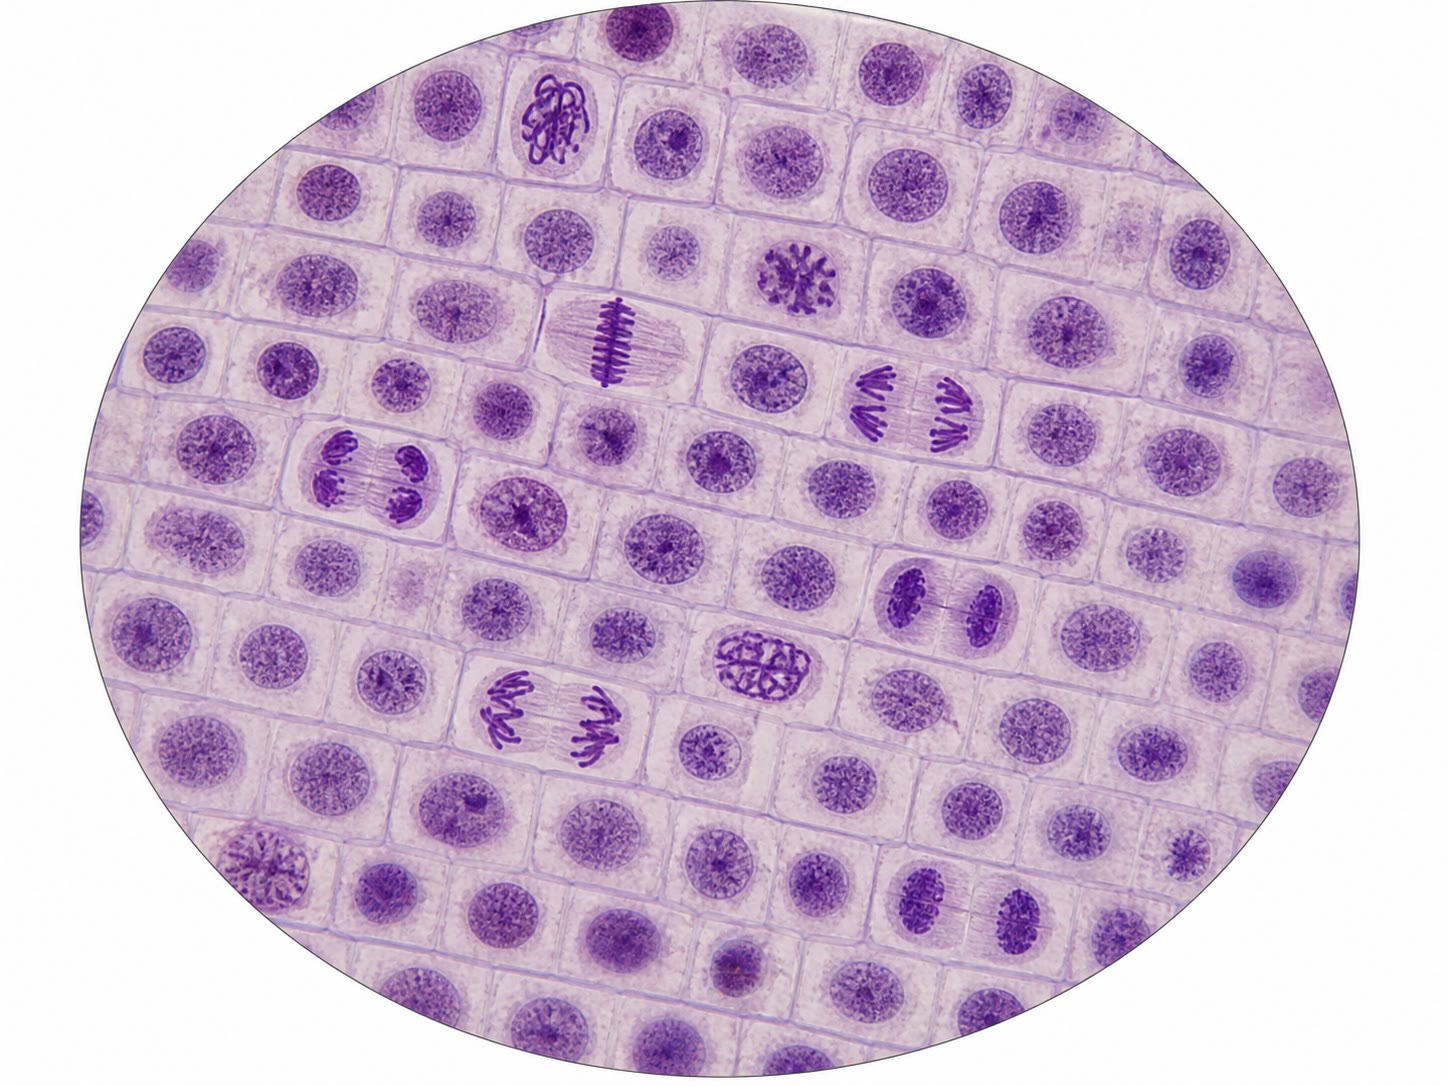
\includegraphics[width=0.58\linewidth]{images/book2/ai/g11-mitosis-root-tip.jpg}

{\small 洋葱根尖压片，置于光学显微镜下观察。大多数
\omterm{def:g10:cells-common-unit:cell}{细胞}处于间期；少数\omterm{def:g10:cells-common-unit:cell}{细胞}呈现凝缩\omterm{def:g11:cell-cycle-mitosis:chromosome}{染色体}，分别处于
\omterm{def:g11:cell-cycle-mitosis:cycle}{有丝分裂}的不同阶段。统计各阶段\omterm{def:g10:cells-common-unit:cell}{细胞}所占的比例，可以测量
各阶段持续的时长。}
\end{omfigure}

\begin{example}[根尖中的计数]\label{ex:g11:cell-cycle-mitosis:count}
在一根根尖中计数 600 个\omterm{def:g10:cells-common-unit:cell}{细胞}，其中 540 个处于间期，60 个处于
\omterm{def:g11:cell-cycle-mitosis:cycle}{有丝分裂}期：\emph{\omterm{def:g11:cell-cycle-mitosis:cycle}{有丝分裂}指数}为 10\%。若\omterm{def:g11:cell-cycle-mitosis:cycle}{细胞周期}为 20 小时，
则\omterm{def:g11:cell-cycle-mitosis:cycle}{有丝分裂}期持续约 $0.10 \times 20 = \qty{2}{h}$；若 60 个分裂\omterm{def:g10:cells-common-unit:cell}{细胞}中有 36 个
处于前期，则前期占这 2 小时的 $36/60$，
约 72 分钟；而仅在 4 个\omterm{def:g10:cells-common-unit:cell}{细胞}中见到的后期约占
8 分钟。最稀少的阶段进行得最快。
\end{example}

\begin{method}[统计染色体与染色单体]\label{met:g11:cell-cycle-mitosis:counting}
对于具有 $2n$ 条\omterm{def:g11:cell-cycle-mitosis:chromosome}{染色体}的\omterm{def:g10:biodiversity-scales:species}{物种}：
\begin{enumerate}
  \item 处于 $\mathrm{G_1}$ 期：$2n$ 条\omterm{def:g11:cell-cycle-mitosis:chromosome}{染色体}，每条含一条\omterm{def:g11:cell-cycle-mitosis:chromosome}{染色单体}，\omterm{def:g10:universal-dna:information}{DNA}
        为 $q$；
  \item S 期之后，经 $\mathrm{G_2}$ 期、前期和中期：$2n$
        条\omterm{def:g11:cell-cycle-mitosis:chromosome}{染色体}，每条含两条\omterm{def:g11:cell-cycle-mitosis:chromosome}{染色单体}（共 $4n$ 条\omterm{def:g11:cell-cycle-mitosis:chromosome}{染色单体}），\omterm{def:g10:universal-dna:information}{DNA} 为 $2q$；
  \item 从后期起：\omterm{def:g10:cells-common-unit:cell}{细胞}内共有 $4n$ 条只含一条\omterm{def:g11:cell-cycle-mitosis:chromosome}{染色单体}的\omterm{def:g11:cell-cycle-mitosis:chromosome}{染色体}，
        每极 $2n$ 条；
  \item 每个子\omterm{def:g10:cells-common-unit:cell}{细胞}：$2n$ 条\omterm{def:g11:cell-cycle-mitosis:chromosome}{染色体}，每条含一条\omterm{def:g11:cell-cycle-mitosis:chromosome}{染色单体}，
        \omterm{def:g10:universal-dna:information}{DNA} 为 $q$。
\end{enumerate}
\omterm{def:g11:cell-cycle-mitosis:chromosome}{着丝粒}一分为二的那一刻，\omterm{def:g11:cell-cycle-mitosis:chromosome}{染色单体}即成为\omterm{def:g11:cell-cycle-mitosis:chromosome}{染色体}。
\end{method}

\begin{example}[人体中的数目]\label{ex:g11:cell-cycle-mitosis:human}
处于中期的人体\omterm{def:g10:cells-common-unit:cell}{细胞}含 46 条\omterm{def:g11:cell-cycle-mitosis:chromosome}{染色体}、92 条\omterm{def:g11:cell-cycle-mitosis:chromosome}{染色单体}；处于后期时
有 92 条\omterm{def:g11:cell-cycle-mitosis:chromosome}{染色体}，每极 46 条；每个子\omterm{def:g10:cells-common-unit:cell}{细胞}含 46 条\omterm{def:g11:cell-cycle-mitosis:chromosome}{染色体}，
每条含一条\omterm{def:g11:cell-cycle-mitosis:chromosome}{染色单体}，所含 \omterm{def:g10:universal-dna:information}{DNA} 与母\omterm{def:g10:cells-common-unit:cell}{细胞}
在其周期开始时完全相同。
\end{example}

\section{有丝分裂的意义}

\begin{proposition}[一致性及其用途]\label{prop:g11:cell-cycle-mitosis:conformity}
由于复制忠实、\omterm{def:g11:cell-cycle-mitosis:cycle}{有丝分裂}精确地分配\omterm{def:g11:cell-cycle-mitosis:chromosome}{染色单体}，
多\omterm{def:g10:cells-common-unit:cell}{细胞}生物体的每个\omterm{def:g10:cells-common-unit:cell}{细胞}都携带与其所来源的受精卵相同的
\omterm{def:g10:universal-dna:information}{遗传信息}。\omterm{def:g11:cell-cycle-mitosis:cycle}{有丝分裂}是生长（胚胎、根尖）、
更新（皮肤、肠道内壁、血液：仅骨髓每天即
生成约 $\num{2e11}$ 个\omterm{def:g10:cells-common-unit:cell}{细胞}）和修复（伤口愈合）的机制；
在单\omterm{def:g10:cells-common-unit:cell}{细胞}真核生物中，它
本身就是繁殖。其调控——进入\omterm{def:g11:cell-cycle-mitosis:cycle}{细胞周期}的决定、
S 期前和后期前的检查——是
\cref{ch:g11:cancer}的主题。
\end{proposition}
\admitted

\begin{remark}[并非所有细胞都会分裂]\label{rem:g11:cell-cycle-mitosis:notall}
大多数神经元和心肌\omterm{def:g10:cells-common-unit:cell}{细胞}在童年早期即离开\omterm{def:g11:cell-cycle-mitosis:cycle}{细胞周期}，
此后不再重新进入。其受损不能通过分裂修复，
这正是脊髓损伤或心脏病发作造成的
持久损失的原因。肝\omterm{def:g10:cells-common-unit:cell}{细胞}在 $\mathrm{G_1}$ 期可静息数月，但
当部分肝脏被切除时，又会重新进入\omterm{def:g11:cell-cycle-mitosis:cycle}{细胞周期}，
数周内即可使器官再生。哪些\omterm{def:g10:cells-common-unit:cell}{细胞}可以分裂、何时分裂，
是机体最严密的调控之一。
\end{remark}

\section{练习}

\begin{exercise}[$\star$]\label{exo:g11:cell-cycle-mitosis:1}
说出\omterm{def:g11:cell-cycle-mitosis:cycle}{细胞周期}的四个时期，并说明每个时期发生的事件。
\end{exercise}

\begin{exercise}[$\star$]\label{exo:g11:cell-cycle-mitosis:2}
定义\omterm{def:g11:cell-cycle-mitosis:chromosome}{染色单体}和\omterm{def:g11:cell-cycle-mitosis:chromosome}{着丝粒}。\omterm{def:g11:cell-cycle-mitosis:chromosome}{染色体}何时
具有两条\omterm{def:g11:cell-cycle-mitosis:chromosome}{染色单体}？
\end{exercise}

\begin{exercise}[$\star$]\label{exo:g11:cell-cycle-mitosis:3}
列出\omterm{def:g11:cell-cycle-mitosis:cycle}{有丝分裂}的四个阶段，并各写出一个关键事件。
\end{exercise}

\begin{exercise}[$\star$]\label{exo:g11:cell-cycle-mitosis:4}
某\omterm{def:g10:cells-common-unit:organelle}{细胞核}含 $1.5q$ 的 \omterm{def:g10:universal-dna:information}{DNA}。该\omterm{def:g10:cells-common-unit:cell}{细胞}处于哪个时期？
\end{exercise}

\begin{exercise}[$\star$]\label{exo:g11:cell-cycle-mitosis:5}
人体\omterm{def:g10:cells-common-unit:cell}{细胞}在
$\mathrm{G_2}$ 期时，有多少条\omterm{def:g11:cell-cycle-mitosis:chromosome}{染色体}和多少条\omterm{def:g11:cell-cycle-mitosis:chromosome}{染色单体}？
\end{exercise}

\begin{exercise}[$\star\star$]\label{exo:g11:cell-cycle-mitosis:6}
根据 \omterm{def:g10:universal-dna:information}{DNA} 含量图，给出各时期的时长，并说明
\omterm{def:g10:cells-common-unit:cell}{细胞}在哪些时期会具有 $2q$ 的 \omterm{def:g10:universal-dna:information}{DNA}。
\end{exercise}

\begin{exercise}[$\star\star$]\label{exo:g11:cell-cycle-mitosis:7}
已知小鼠 $2n = 40$。求
中期\omterm{def:g10:cells-common-unit:cell}{细胞}、后期\omterm{def:g10:cells-common-unit:cell}{细胞}（整个\omterm{def:g10:cells-common-unit:cell}{细胞}）及子\omterm{def:g10:cells-common-unit:cell}{细胞}中的
\omterm{def:g11:cell-cycle-mitosis:chromosome}{染色体}数和\omterm{def:g11:cell-cycle-mitosis:chromosome}{染色单体}数。
\end{exercise}

\begin{exercise}[$\star\star$]\label{exo:g11:cell-cycle-mitosis:8}
在一根根尖中计数 800 个\omterm{def:g10:cells-common-unit:cell}{细胞}：间期 720 个，前期 48 个，
中期 16 个，后期 6 个，末期 10 个。计算\omterm{def:g11:cell-cycle-mitosis:cycle}{有丝分裂}指数，
并假设\omterm{def:g11:cell-cycle-mitosis:cycle}{细胞周期}为 24 小时，求各阶段的时长。
\end{exercise}

\begin{exercise}[$\star\star$]\label{exo:g11:cell-cycle-mitosis:9}
秋水仙碱是从秋水仙中提取的一种药物，
能阻止纺锤体的形成。预测用它处理的分裂\omterm{def:g10:cells-common-unit:cell}{细胞}会发生什么变化，
并说明生物学家为什么用它来制备\omterm{def:g11:cell-cycle-mitosis:chromosome}{核型}。
\end{exercise}

\begin{exercise}[$\star\star$]\label{exo:g11:cell-cycle-mitosis:10}
解释\omterm{def:g11:cell-cycle-mitosis:chromosome}{染色体}为什么必须先凝缩才能被移动，以及
分开之后为什么又会解螺旋。
\end{exercise}

\begin{exercise}[$\star\star$]\label{exo:g11:cell-cycle-mitosis:11}
受精卵在最初几天每 12 小时分裂一次。
5 天后共有多少个\omterm{def:g10:cells-common-unit:cell}{细胞}？每次分裂是否都需要完整的
$\mathrm{G_1}$ 期？
\end{exercise}

\begin{exercise}[$\star\star\star$]\label{exo:g11:cell-cycle-mitosis:12}
在后期，某条\omterm{def:g11:cell-cycle-mitosis:chromosome}{染色体}的两条\omterm{def:g11:cell-cycle-mitosis:chromosome}{染色单体}未能分开，
并且都移向同一极。描述由此形成的两个子\omterm{def:g10:cells-common-unit:cell}{细胞}（\omterm{def:g11:cell-cycle-mitosis:chromosome}{染色体}
数、\omterm{def:g10:universal-dna:information}{DNA} 含量），并说明为什么这种错误在体\omterm{def:g10:cells-common-unit:cell}{细胞}中通常
没有后果，但在某些情况下却很严重。
\end{exercise}

\begin{exercise}[$\star\star\star$]\label{exo:g11:cell-cycle-mitosis:13}
骨髓每天生成 $\num{2e11}$ 个血\omterm{def:g10:cells-common-unit:cell}{细胞}。若骨髓
前体\omterm{def:g10:cells-common-unit:cell}{细胞}的\omterm{def:g11:cell-cycle-mitosis:cycle}{细胞周期}为 24 小时，估算任一时刻正在分裂的
前体\omterm{def:g10:cells-common-unit:cell}{细胞}数，并讨论一种阻断\omterm{def:g11:cell-cycle-mitosis:cycle}{有丝分裂}的药物在一周内
会对血液产生什么影响。
\end{exercise}

\begin{exercise}[$\star\star\star$]\label{exo:g11:cell-cycle-mitosis:14}
解释为什么制备\omterm{def:g11:cell-cycle-mitosis:chromosome}{核型}时，应选取中期阻滞的\omterm{def:g10:cells-common-unit:cell}{细胞}，
而不是间期或后期的\omterm{def:g10:cells-common-unit:cell}{细胞}。
\end{exercise}

\begin{exercise}[$\star\star\star$]\label{exo:g11:cell-cycle-mitosis:15}
肝脏被切除了三分之二，三周内又重新长回。利用
\omterm{def:g11:cell-cycle-mitosis:cycle}{细胞周期}描述其\omterm{def:g10:cells-common-unit:cell}{细胞}发生了什么变化，并说明第 3 天与第 0 天
相比，肝\omterm{def:g10:cells-common-unit:cell}{细胞}的 \omterm{def:g10:universal-dna:information}{DNA} 含量有何不同。
\end{exercise}

\section{问题：根尖的时间表}

\begin{problem}[{周末问题——逐个细胞计数的根尖：
细胞周期中每个阶段的长度、每一时刻的 DNA 含量、
根一天产生的细胞数，以及后期的八分钟}]
\label{pb:g11:cell-cycle-mitosis:1}
一个班级压片并染色一根大蒜根尖（$2n = 16$），在生长区
计数 1000 个\omterm{def:g10:cells-common-unit:cell}{细胞}：间期 900 个，前期 60 个，中期 18 个，
后期 8 个，末期 14 个。独立测量得知，这些\omterm{def:g10:cells-common-unit:cell}{细胞}的\omterm{def:g11:cell-cycle-mitosis:cycle}{细胞周期}
为 20 小时。取生长区
含 20\,000 个\omterm{def:g10:cells-common-unit:cell}{细胞}。

\medskip
\noindent\textbf{第一部分——\omterm{def:g11:cell-cycle-mitosis:cycle}{有丝分裂}指数。}
\begin{enumerate}
  \item 计算该组织的\omterm{def:g11:cell-cycle-mitosis:cycle}{有丝分裂}指数。
  \item 假设某阶段\omterm{def:g10:cells-common-unit:cell}{细胞}所占的比例等于该阶段占\omterm{def:g11:cell-cycle-mitosis:cycle}{细胞周期}的
        比例，计算
        \omterm{def:g11:cell-cycle-mitosis:cycle}{有丝分裂}的时长。
  \item 计算四个阶段各自的时长。
  \item 哪一个阶段最短？推测它为何能如此迅速。
  \item 为什么该方法需要计数大量\omterm{def:g10:cells-common-unit:cell}{细胞}，
        且这些\omterm{def:g10:cells-common-unit:cell}{细胞}必须只来自生长区？
\end{enumerate}

\medskip
\noindent\textbf{第二部分——\omterm{def:g11:cell-cycle-mitosis:chromosome}{染色体}与 \omterm{def:g10:universal-dna:information}{DNA}。}
\begin{enumerate}[resume]
  \item 处于中期的大蒜\omterm{def:g10:cells-common-unit:cell}{细胞}含有多少条\omterm{def:g11:cell-cycle-mitosis:chromosome}{染色体}，
        以及多少条\omterm{def:g11:cell-cycle-mitosis:chromosome}{染色单体}？
  \item 后期\omterm{def:g10:cells-common-unit:cell}{细胞}中有多少条\omterm{def:g11:cell-cycle-mitosis:chromosome}{染色体}在移动，
        其中每一极各有多少条？
  \item 设 $q$ 为子\omterm{def:g10:cells-common-unit:cell}{细胞}的 \omterm{def:g10:universal-dna:information}{DNA} 含量，
        给出前期\omterm{def:g10:cells-common-unit:cell}{细胞}、后期\omterm{def:g10:cells-common-unit:cell}{细胞}（整个\omterm{def:g10:cells-common-unit:cell}{细胞}）和末期
        \omterm{def:g10:cells-common-unit:cell}{细胞}（每个\omterm{def:g10:cells-common-unit:organelle}{细胞核}）的 \omterm{def:g10:universal-dna:information}{DNA} 含量。
  \item 在 900 个间期\omterm{def:g10:cells-common-unit:cell}{细胞}中，若 $\mathrm{G_1}$、S 和 $\mathrm{G_2}$ 期
        分别为 8、7 和 4 小时，则约有多少个\omterm{def:g10:cells-common-unit:cell}{细胞}处于 S 期？
  \item 某学生发现一个\omterm{def:g10:cells-common-unit:cell}{细胞}，其中 32 条单\omterm{def:g11:cell-cycle-mitosis:chromosome}{染色单体}的\omterm{def:g11:cell-cycle-mitosis:chromosome}{染色体}
        散布于\omterm{def:g10:cells-common-unit:cell}{细胞质}中。该\omterm{def:g10:cells-common-unit:cell}{细胞}处于哪一阶段，
        刚刚发生了什么？
\end{enumerate}

\medskip
\noindent\textbf{第三部分——根的产出。}
\begin{enumerate}[resume]
  \item 若生长区每个\omterm{def:g10:cells-common-unit:cell}{细胞}的\omterm{def:g11:cell-cycle-mitosis:cycle}{细胞周期}均为 20 小时，
        则该区每小时产生多少个新\omterm{def:g10:cells-common-unit:cell}{细胞}？
  \item 每个新\omterm{def:g10:cells-common-unit:cell}{细胞}离开生长区后，伸长至约
        \qty{100}{\micro m}。在宽度为一个\omterm{def:g10:cells-common-unit:cell}{细胞}的一列\omterm{def:g10:cells-common-unit:cell}{细胞}中，
        根每天伸长多少？与观测到的
        每天 \qty{1}{mm} 相比，并解释其差异。
  \item 每个子\omterm{def:g10:cells-common-unit:cell}{细胞}必须复制 $2n = 16$ 条\omterm{def:g11:cell-cycle-mitosis:chromosome}{染色体}，共
        $\num{1.6e10}$ 个碱基对。若\omterm{prop:g11:dna-replication:forks}{复制叉}每秒移动 50 个\omterm{def:g10:universal-dna:nucleotide}{核苷酸}，
        则需要多少个复制起点，才能在 S 期的 7 小时内
        完成复制？
  \item 将根放入低温（\qty{4}{\celsius}）环境中一天。
        预测计数结果的变化，以及若低温使所有阶段
        同等减慢，\omterm{def:g11:cell-cycle-mitosis:cycle}{有丝分裂}指数会如何变化。
  \item 一种除草剂阻断 \omterm{def:g10:universal-dna:information}{DNA} 聚合酶。一天后，压片中
        仍能看到哪些阶段，哪些阶段已经消失？
        请说明理由。
\end{enumerate}

\medskip
\noindent\textbf{第四部分——计数的结论。}
\begin{enumerate}[resume]
  \item 另一个班级对同一组织进行计数，在 1000 个\omterm{def:g10:cells-common-unit:cell}{细胞}中
        发现 4 个后期\omterm{def:g10:cells-common-unit:cell}{细胞}。他们算出的时长是多少？这种分歧对于
        只在少数\omterm{def:g10:cells-common-unit:cell}{细胞}中出现的阶段是否令人意外？
  \item 合并两个班级的数据（2000 个\omterm{def:g10:cells-common-unit:cell}{细胞}，12 个后期\omterm{def:g10:cells-common-unit:cell}{细胞}），
        重新计算后期的时长。
  \item 培养的人体\omterm{def:g10:cells-common-unit:cell}{细胞}\omterm{def:g11:cell-cycle-mitosis:cycle}{有丝分裂}指数为 4\%，\omterm{def:g11:cell-cycle-mitosis:cycle}{细胞周期}为
        24 小时。比较其\omterm{def:g11:cell-cycle-mitosis:cycle}{有丝分裂}的时长与
        大蒜的时长。
  \item 解释为什么肿瘤的\omterm{def:g11:cell-cycle-mitosis:cycle}{有丝分裂}指数往往为其
        来源组织的数倍，以及这对
        作用于纺锤体的药物意味着什么。
  \item 陈述结论：大蒜根尖\omterm{def:g10:cells-common-unit:cell}{细胞}的\omterm{def:g11:cell-cycle-mitosis:cycle}{细胞周期}时间表，
        逐阶段列出，并指出哪一阶段的八分钟决定了
        每个子\omterm{def:g10:cells-common-unit:cell}{细胞}获得十六条\omterm{def:g11:cell-cycle-mitosis:chromosome}{染色体}。
\end{enumerate}
\end{problem}
